\chapter{Diseño e implementación} % Main chapter title

\label{Chapter3} % Change X to a consecutive number; for referencing this chapter elsewhere, use \ref{ChapterX}

\definecolor{mygreen}{rgb}{0,0.6,0}
\definecolor{mygray}{rgb}{0.5,0.5,0.5}
\definecolor{mymauve}{rgb}{0.58,0,0.82}

%%%%%%%%%%%%%%%%%%%%%%%%%%%%%%%%%%%%%%%%%%%%%%%%%%%%%%%%%%%%%%%%%%%%%%%%%%%%%
% parámetros para configurar el formato del código en los entornos lstlisting
%%%%%%%%%%%%%%%%%%%%%%%%%%%%%%%%%%%%%%%%%%%%%%%%%%%%%%%%%%%%%%%%%%%%%%%%%%%%%
\lstset{ %
  backgroundcolor=\color{white},   % choose the background color; you must add \usepackage{color} or \usepackage{xcolor}
  basicstyle=\footnotesize,        % the size of the fonts that are used for the code
  breakatwhitespace=false,         % sets if automatic breaks should only happen at whitespace
  breaklines=true,                 % sets automatic line breaking
  captionpos=b,                    % sets the caption-position to bottom
  commentstyle=\color{mygreen},    % comment style
  deletekeywords={...},            % if you want to delete keywords from the given language
  %escapeinside={\%*}{*)},          % if you want to add LaTeX within your code
  %extendedchars=true,              % lets you use non-ASCII characters; for 8-bits encodings only, does not work with UTF-8
  %frame=single,	                % adds a frame around the code
  keepspaces=true,                 % keeps spaces in text, useful for keeping indentation of code (possibly needs columns=flexible)
  keywordstyle=\color{blue},       % keyword style
  language=[ANSI]C,                % the language of the code
  %otherkeywords={*,...},           % if you want to add more keywords to the set
  numbers=left,                    % where to put the line-numbers; possible values are (none, left, right)
  numbersep=5pt,                   % how far the line-numbers are from the code
  numberstyle=\tiny\color{mygray}, % the style that is used for the line-numbers
  rulecolor=\color{black},         % if not set, the frame-color may be changed on line-breaks within not-black text (e.g. comments (green here))
  showspaces=false,                % show spaces everywhere adding particular underscores; it overrides 'showstringspaces'
  showstringspaces=false,          % underline spaces within strings only
  showtabs=false,                  % show tabs within strings adding particular underscores
  stepnumber=1,                    % the step between two line-numbers. If it's 1, each line will be numbered
  stringstyle=\color{mymauve},     % string literal style
  tabsize=2,	                   % sets default tabsize to 2 spaces
  title=\lstname,                  % show the filename of files included with \lstinputlisting; also try caption instead of title
  morecomment=[s]{/*}{*/}
}
En este capítulo se enumeran y desarrollan los aspectos considerados a la hora diseñar el robot. Se tuvieron en cuenta los alcances establecidos como así también las posibilidades económicas de solventar el proyecto.
%----------------------------------------------------------------------------------------
%	SECTION 1
%----------------------------------------------------------------------------------------
\section{Diseño de hardware}

En esta sección se detallan los componentes y módulos electrónicos que forman parte del robot. Se detalla la función que desempeña cada uno de ellos. En la figura \ref{fig:diagramaini} se puede apreciar un diagrama en bloques de los módulos que conforman el robot.


\begin{figure}[h]
	\centering
	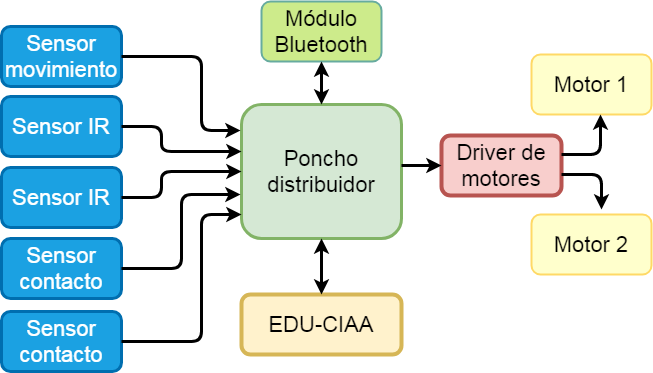
\includegraphics[width=12cm]{./Figures/diagini.PNG}
	\caption{Diagrama en bloques del robot.}
	\label{fig:diagramaini}
\end{figure}



	\subsection{Poncho}
Se denominación  “Poncho”  se utiliza entre la comunidad del proyecto CIAA para referirse a una  placa de expansión de “Shield”  que se conecta sobre algún procesador de la familia CIAA.  Para este proyecto se diseñó un poncho para facilitar las conexiones de la placa EDU-CIAA con los sensores, actuadores y el módulo de comunicación bluetooth.

		\subsubsection{Diseño esquemático del poncho}

El poncho consta de conectores para las señales de entrada:

\begin{itemize}
	\item Sensores infrarrojos (2).
	\item finales de carrera (2).
	\item sensor de movimiento (1).
\end{itemize}

A su vez, permite la conexión con los dispositivos de salida

\begin{itemize}
	\item Módulo de control de motores.
	\item Relé actuador (en la placa).
	\item Buzzer y LEDs (en la placa).
\end{itemize}

La placa posee conexionado para montar un módulo HC-05 de comunicación bluetooth y un conector destinado a dispositivos I2C (como podría ser un módulo de girósocpo o acelerómetro).

		\subsubsection{Diseño PCB del poncho}


La placa fue diseñada durante la cursada de la asignatura “diseño de circuitos s, según los lineamientos expuestos en la documentación para ponchos CIAA. Se procedió a la fabricación de la placa utilizando medios caseros de manufactura.

El diseño de PCB se realizó con el software KiCad \citep{KiCad} (Versión 5.1.9), el cual es un paquete de software para el diseño de circuitos electrónicos o EDA (Electronic Design
Automation). En la figura \ref{fig:poncho3d} se observa el modelo 3D de la placa y sus componentes.


\begin{figure}[h]
	\centering
	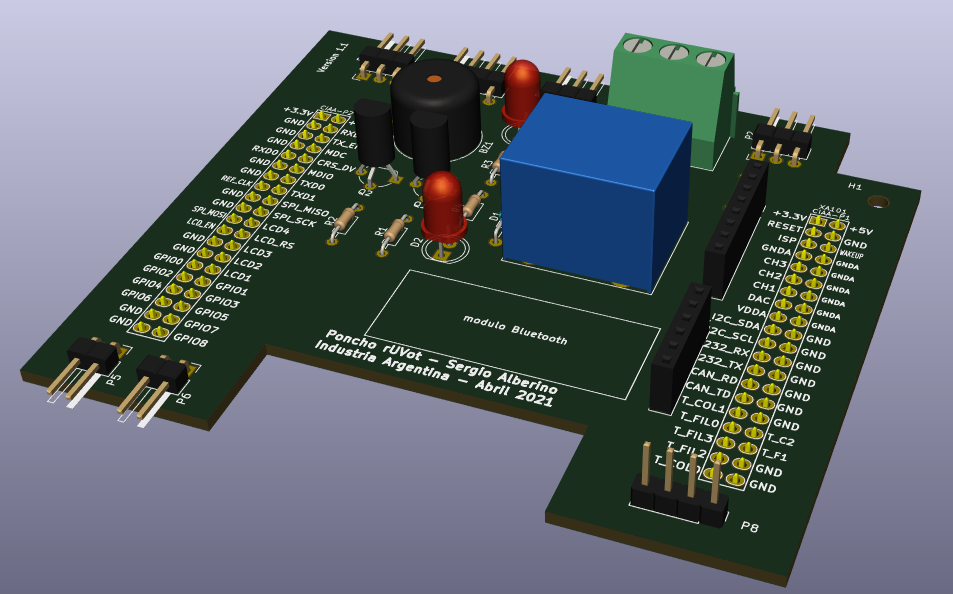
\includegraphics[width=11cm]{./Figures/ponchoiso.PNG}
	\caption{Vista del modelo 3D del poncho rUVot.}
	\label{fig:poncho3d}
\end{figure}


En la figura \ref{fig:esquematico} se presenta el circuito esquemático del poncho donde se puede observar el conexionado eléctrico.

%\begin{figure}[h]
%	\centering
%	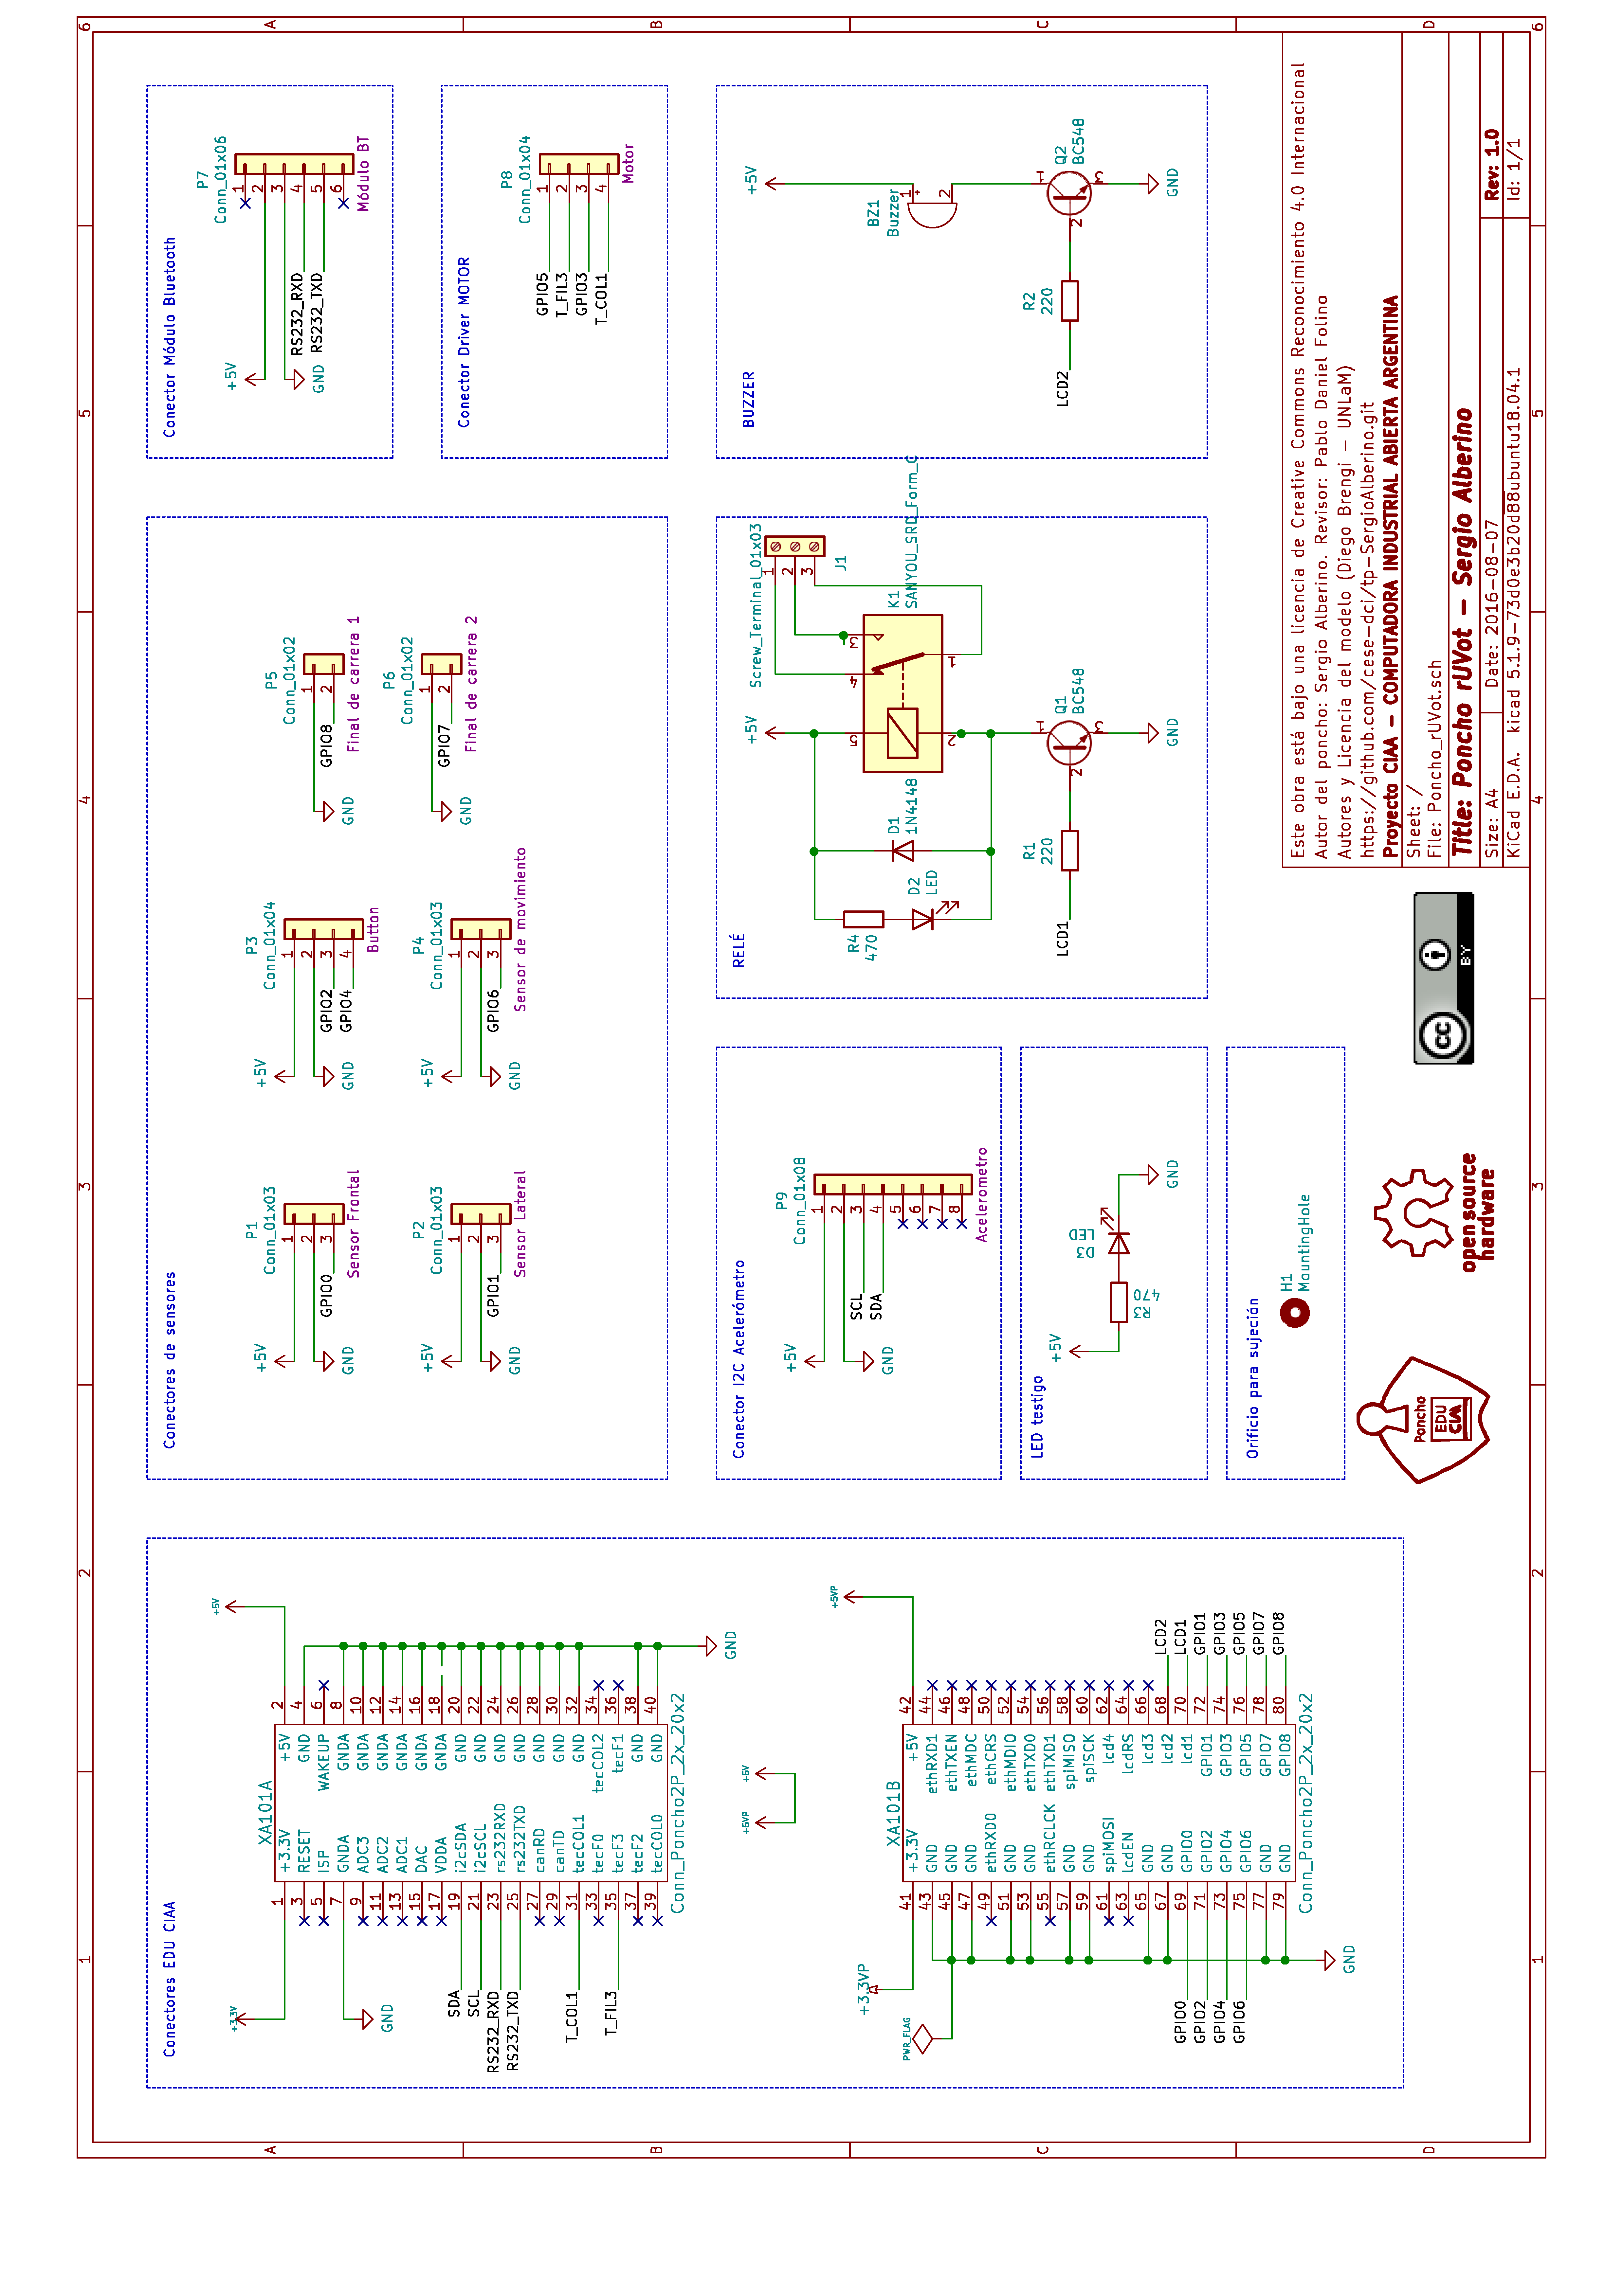
\includegraphics[width=\textwidth]{./Figures/esquematico.png}
%	\caption{Circuito esquemático del poncho.}
%	\label{fig:esquematico}
%\end{figure}
%\pagebreak

\subsection{Esquema de  de comunicaciones}

\section{Diseño mecánico}
\subsection{Gabinete del robot}
\subsection{Motores}

\section{Diseño de software}
\subsection{Tarea de control de motores}
\subsection{Tarea de comunicaciones}







%
%
%
%
%\begin{verbatim}
%\begin{lstlisting}[caption= "un epígrafe descriptivo"]
%	las líneas de código irían aquí...
%\end{lstlisting}
%\end{verbatim}
%
%A modo de ejemplo:
%
%\begin{lstlisting}[label=cod:vControl,caption=Pseudocódigo del lazo principal de control.]  % Start your code-block
%
%#define MAX_SENSOR_NUMBER 3
%#define MAX_ALARM_NUMBER  6
%#define MAX_ACTUATOR_NUMBER 6
%
%uint32_t sensorValue[MAX_SENSOR_NUMBER];		
%FunctionalState alarmControl[MAX_ALARM_NUMBER];	//ENABLE or DISABLE
%state_t alarmState[MAX_ALARM_NUMBER];						//ON or OFF
%state_t actuatorState[MAX_ACTUATOR_NUMBER];			//ON or OFF
%
%void vControl() {
%
%	initGlobalVariables();
%	
%	period = 500 ms;
%		
%	while(1) {
%
%		ticks = xTaskGetTickCount();
%		
%		updateSensors();
%		
%		updateAlarms();
%		
%		controlActuators();
%		
%		vTaskDelayUntil(&ticks, period);
%	}
%}
%\end{lstlisting}



